\documentclass[11pt]{article}
\usepackage{geometry}
\usepackage{graphics}
\usepackage{graphicx}
\usepackage{amssymb}
\usepackage{amstext}
\usepackage{color}
\usepackage{amsmath}
\usepackage[ngerman]{babel}
\usepackage[latin1]{inputenc}
\usepackage{units}
\usepackage{algorithm}
\usepackage{algorithmic}
\geometry{a4paper,left=20mm,right=10mm, top=13mm, bottom=20mm}
\newcommand{\ff}{\triangleright}
\author{Robert Hartmann}
\begin{document}
$$L\triangleright W = \bigcup_{u\in L} u\triangleright W$$
\vspace{5mm}
$$u\triangleright W := Min_{\sqsubseteq} \{w:w\in W \wedge u\sqsubseteq w\}$$
\textbf{\large{Frage: 1}}\\\\
Sei $$L_1=\{a,ab,aab,aaab,abbb,abb\}$$
Baum: (bez�glich $\sqsubseteq$)\\
\begin{center}
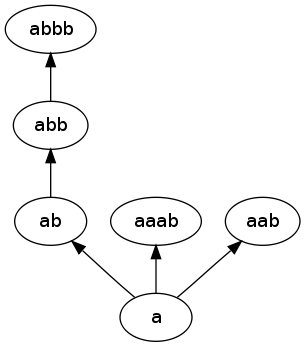
\includegraphics[scale=0.4]{baum.png}
\end{center}
Nun gibt es die Frage was der Ausdruck $a\ff L_1$ ist.\\\\
Erste Idee:
$$a\ff L_1 = \{ab,aaab,aab\}$$
also quasi die erste Stufe des Baumes.\\
Bei genauerer Betrachtung steht ja $\sqsubseteq$ da und nicht $\sqsubset$.
Daher m�sste doch eigentlich:
$$a\ff L_1 = \{a\}$$ sein, weil in dem Fall $a$ das kleinste Pr�fix von allen
W�rtern aus $L_1$ ist.\\
Was davon ist richtig?\\\\
Sollte der letztere Fall der richtige sein, dann gilt scheinbar generell:
$$\text{Aus }u\in L\text{ folgt: }u\ff L=\{u\}$$
\end{document}
